% TODO: add in a version and date info
% TODO: operation section, led status codes
% TODO: Programmer Info copy this from the regulator datasheet and ftdi datasheet about current sourcing, drive strength electrical specs mechanical specs on the programming connector 0.1" spacing, mating connector, etc} supported baud rates
% TODO: also include recommended land pattern for programmer header (smd and through hole) also reference recommended programming cable
% TODO: add in pdf schematic

\documentclass[10pt,letterpaper]{datasheet}

\usepackage{amssymb}
\usepackage{color}
\usepackage{graphicx}
\usepackage{subfig}
\usepackage{lipsum}
\usepackage{multicol}
% \usepackage[small]{subfigure}
\usepackage{tabularx}

\newlength\SUBSIZE
\newcommand{\mbp}{MSP430~BSL~Programmer}
\newcommand{\PID}{FCD-PRG01}
\newcommand{\PIDCBL}{FCD-CBL01}
\newcommand{\fcd}{Flying~Camp~Design}
\newcommand{\FCD}{FLYING~CAMP~DESIGN}
\newcommand{\fcdurl}{\href{http://www.flyingcampdesign.com}%
                          {www.flyingcampdesign.com}}
\newcommand{\tos}{\texttt{TinyOS}}
\newcommand{\fixme}{{\color{red}{---FIXME---}}}

\pagestyle{fancy}
\lfoot{\fcdurl}
\cfoot{\PID\ Datasheet -- Rev. A}

\usepackage[pdftex,
            colorlinks=true, 
            urlcolor=blue, 
            hyperfootnotes=true,
            bookmarks=true,
            bookmarksopen=false,
            pdfpagemode=None]{hyperref}
\hypersetup{pdftitle={\PID\ Datasheet},
            pdfauthor={\FCD},
            pdfkeywords={msp430,BSL,bootstrap,loader,programmer}}

\begin{document}
\title{\color{red}{\bf \mbp\newline\PID}}
\author{\FCD}
\date{}
\maketitle
\makefooter
\thispagestyle{fancy}

\section*{Highlights}
\begin{multicols}{2}
  \begin{itemize}
    \item MSP430 F1x, F2x, F4x, F5x compatible%
    \footnote{MSPGCC BSL tools currently support F1x, F2x, and F4x only}
    \item Standard 6 pin, 0.1" header interface
    \item USB bus powered
    \item 3.3V target supply output (up to 400mA)
    \item Cross platform driver support for Windows, Linux, and Mac OS
    \item Full MSPGCC GNU toolchain support
    \item Full \tos\ support
    \item Fully Open-Source hardware design%
    \footnote{Design files available at %
    \href{http://www.flyingcampdesign.com/msp430-bsl-programmer.html}%
         {http://www.flyingcampdesign.com/msp430-bsl-programmer.html}}
  \end{itemize}
\end{multicols}

\section*{Product Description}
\begin{multicols}{2}
  The \PID\ is a USB bootstrap loader\footnote{``MSP430 Programming Via the Bootstrap Loader'' Application Note  (\href{http://www-s.ti.com/sc/techlit/slau265}{http://www-s.ti.com/sc/techlit/slau265})} (BSL) programmer for the Texas Instruments MSP430 microprocessor.  For designs where low cost or small form factor prohibit the integration of custom programming logic or a large JTAG header, the \PID\ enables in-system programming by including a single 6 pin header in the target device design.
  
  \begin{center}
    
\includegraphics[width=3 in]{fcd-prg01-diag}
  \end{center}
  
  Designed to work with the cross platform MSPGCC toolchain, the \PID\ provides an open source, cross platform alternative to platform dependent development tools for the MSP430 microprocessor.
  
  \begin{center}
    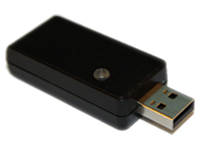
\includegraphics[width=2 in]{fcd-prg01}
  \end{center}
  
  The \PID\ integrates a USB-to-serial converter and on board regulated power supply into a small USB dongle, allowing programming and test capability over a single interface.  It exposes a standard 6 pin, 0.1" header which can be used to interface to the target board via a device specific cable harness.  This modular aproach provides designers with the flexibility to select the optimal physical programming interface for the unique design constraints of each target platform.  

\end{multicols}

\section*{Ordering Information}
\begin{flushleft}
  \label{tab:ordering}
  \begin{tabular}{l l}
    \textbf{\PID} & \mbp \\
    \textbf{FCD-CBL01} & Programming interface cable (6x1, 0.1" $\leftrightarrow$ 3x2, 2mm) \\
  \end{tabular}
\end{flushleft}

\newpage

\section*{Programming Interface}
\begin{flushleft}
  The \PID\ provides a standard 6x1, 0.1" programming header for powering and communicating with the target device. \\

  \begin{figure}[!h]
    \label{fig:fcd-prg01-pinout}
    \begin{center}
      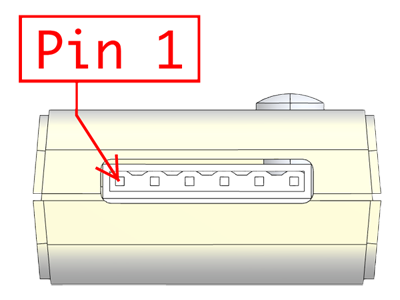
\includegraphics[width=2 in]{fcd-prg01-pinout}
    \end{center}
    \caption{6x1, 0.1" Header}
  \end{figure}
  
  \subsection*{Pinout}
  \begin{flushleft}
    \label{tab:pinout}
    \begin{tabular}{|c|c|c|c|}
      \hline
      \PID\ Signal &
      \PID\  Pin &
      MSP430 devices with TEST pin &
      MSP430 devices without TEST pin \\
      \hline
      DTR & 1 & TEST & TCK \\
      RXD & 2 & UART\_TX & UART\_TX \\
      TXD & 3 & UART\_RX & UART\_RX \\
      VCC & 4 & VDD & VDD \\
      RTS & 5 & RST/NMI & RST/NMI \\
      GND & 6 & GND & GND \\
      \hline
    \end{tabular}
  \end{flushleft}

  \bigskip

  \subsection*{Electrical Characteristics}
    \subsubsection*{VCC Target Supply Output (Pin 4)}
    \label{tab:elec-sup}
    \begin{tabular}{|l|c|c|c|c|c|}
      \hline
      Parameter &
      Minimum &
      Typical &
      Maximum &
      Units &
      Conditions \\
      \hline
      Output Voltage & - & 3.3 & - & V & \\
      Output Current & - & - & 0.4 & A & \\
      Short Circuit Current & - & 450 & - & mA & Vout = 0 V \\
      Dropout Voltage & - & 75 & 200 & mV & Iout = 400 mA \\
      Accuracy & - & 1 & - & \% & \\
      \hline
    \end{tabular}
  
    \subsubsection*{UART and I/O (Pins 1,2,3,5)}
    \label{tab:elec-io}
    \begin{tabular}{|l|c|c|c|c|c|}
      \hline
      Parameter &
      Minimum &
      Typical &
      Maximum &
      Units &
      Conditions \\
      \hline
      DC Input Voltage & -0.5 & - & 3.8 & V & \\
      Output Drive Strength & - & 12 & - & mA & \\
      Output Voltage High & 2.2 & 2.8 & 3.2 & V & Isource = 3 mA \\
      Output Voltage Low & 0.3 & 0.4 & 0.6 & V & Isink = 8 mA \\
      Input Switching Threshold & 1.0 & 1.2 & 1.5 & V & \\
      Input Switching Hysteresis & 20 & 25 & 30 & mV & \\
      \hline
    \end{tabular}
\end{flushleft}
  
\newpage
  
\section*{Programming Cables}
\subsection*{\PIDCBL}
\begin{flushleft}
  A programming cable harness which mates with standard 3x2, 2mm PCB headers is available from \fcd\ for use with the \PID.
  
  \begin{figure}[!h]
    \label{fig:fcd-cbl01}
    \begin{center}
      
\includegraphics[]{fcd-cbl01}
    \end{center}
    \caption{Flying Camp Design FCD-CBL01}
  \end{figure}
  
  \fcd\ recommends using the following through hole and surface mount headers for use with the \PIDCBL:
  
  \begin{figure}[!h]
    \label{fig:rec-prog-hdr}
    \begin{center}
      \subfloat[\href{http://www.hirose.co.jp/cataloge_hp/e54305002.pdf}%
                     {Hirose DF11-6DP-2DSA(01)}]{
        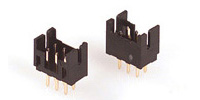
\includegraphics[width=2 in]{DF11-6DP-2DSA(01)_sml}}
      \subfloat[\href{http://www.hirose.co.jp/cataloge_hp/e54305002.pdf}%
                     {Hirose DF11G-6DP-2V(50)}]{
        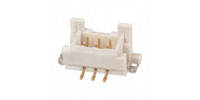
\includegraphics[width=2 in]{DF11G-6DP-2V(50)_sml}}
      \caption{Recommended headers for use with the \PIDCBL\ cable}
    \end{center}
  \end{figure}
  
  A Cadsoft Eagle CAD library which contains land pattern footprints for these headers is available for download on the \PID\ product page: %
  \href{http://www.flyingcampdesign.com/msp430-bsl-programmer.html}%
       {http://www.flyingcampdesign.com/msp430-bsl-programmer.html} \newline

\subsection*{Custom Programming Cables}
  For those customers wishing to design their own custom programming cables, \fcd\ recommends the following mating connector for use with the 6 pin programming interface:

  \begin{figure}[!h]
    \label{fig:50-57-9006}
    \begin{center}
      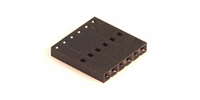
\includegraphics[width=2 in]{50-57-9006_sml}
    \end{center}
    \caption{\href{http://www.molex.com/pdm_docs/sd/050579006_sd.pdf}%
                  {Molex 50-57-9006}}
  \end{figure}

\end{flushleft}

\newpage

\section*{Installation}
\begin{flushleft}
  The \PID\ uses a USB $\leftrightarrow$ Serial interface chip (\href{http://ftdichip.com/Products/FT232R.htm}{FTDI Chip FT232R}) and corresponding operating system driver to provide a Virtual COM Port (VCP) interface layer to the BSL programming software.  The BSL programming software depends upon this VCP interface layer to control the communication pins on the programmer.\\
  \begin{enumerate}
    \item \textbf{Before plugging in the \PID\ to your computer}, install the appropriate driver for your operating system by following the corresponding installation guide available online at: \newline
    \href{http://ftdichip.com/Documents/InstallGuides.htm}{http://ftdichip.com/Documents/InstallGuides.htm} \newline

    A full listing of the latest VCP drivers for all supported operating systems is available online at: \newline \href{http://ftdichip.com/Drivers/VCP.htm}{http://ftdichip.com/Drivers/VCP.htm} \newline

    \textbf{Note:} A Linux driver for the FT232R is included in most newer kernels ( $>$ 2.4.20 or greater).  However, on some kernels an older F232BM driver may be used which is compatible with the FT232R.  \newline

    \item After installing the appropriate driver for your operating system, insert the \PID\ into a free USB port on your computer.

    \item If installation was successful, the \PID\ should appear as a VCP on your computer:
    
    \label{tab:elec-io}
    \begin{tabular}{l l}
      \textbf{Windows} & COM[X] \\
      \textbf{Linux} & /dev/ttyUSB[X] \\
      \textbf{Mac OS X} & /dev/tty.usbserial-[...] \\
    \end{tabular}
  \end{enumerate}
\end{flushleft}

\newpage

\section*{Software Support}
\begin{flushleft}
The Virtual COM Port (VCP) drivers provide a serial port interface to the BSL control software.  This generic software interface enables the use of third party BSL tools, as well as provides a simple abstraction to those users wishing to write their own BSL tools.  The mapping between the VCP signal and the programmer pins is shown in the table on page~\pageref{tab:pinout}.  The following examples show how to use the \PID\ with the BSL tools available from a couple popular MSP430 toolchains.

\subsection*{MSPGCC Toolchain Programming Example}
The MSPGCC GNU toolchain includes a set of python scripts (``tools''\footnote{\href{http://mspgcc.sourceforge.net/tools.html}{http://mspgcc.sourceforge.net/tools.html}}) which can be used to control the MSP430 BSL (download to Flash and/or RAM, erase, verify, etc) on supported flash devices.  The following example clears all flash memory, programs the target with the Intel hex firmware file ``firmware.ihex'', and then resets the target:
\begin{verbatim}
    python msp430-bsl.py --speed=9600 --swap-reset-test --invert-reset --invert-test \
    -c /dev/path-to-msp430-bsl-programmer -r -e -I -p path/to/firmware.ihex
\end{verbatim}
More information about msp430-bsl.py is available online at: \href{http://mspgcc.sourceforge.net/tools.html\#pybsl}{http://mspgcc.sourceforge.net/tools.html\#pybsl}

\subsection*{TinyOS Programming Example}
The \tos\ toolchain includes built in support for the \PID.  The following example can be used to compile a \tos\ application and install it onto an MSP430 based \tos\ ``platform'':
\begin{verbatim}
    make [platform] install miniprog
\end{verbatim}
More information about the \tos\ toolchain is available online at: \href{http://tinyos.net}{http://tinyos.net}
\end{flushleft}

\subsection*{MSP430 BSL Utility}
The \fcd\ MSP430 BSL Utility is an open source, cross-platform GUI utility which was designed to be fully compatible with the \PID. More information about using the \PID\ with this software is available on the MSP430 BSL Utility product page: \newline
\href{http://www.flyingcampdesign.com/msp430-bsl-utility.html}{http://www.flyingcampdesign.com/msp430-bsl-utility.html}

\newpage

\section*{Questions?}
Contact %
\href{mailto:support@flyingcampdesign.com}%
     {support@flyingcampdesign.com} %
or visit %
\href{http://www.flyingcampdesign.com/support.html}%
     {http://www.flyingcampdesign.com/support.html}

\newpage

\section*{Legal}

\begin{flushleft}
Flying Camp Design reserves all rights to this document and the information
contained herein.  Product names, trademarks, or logos described or
displayed herein may be subject to Flying Camp Design or third-party
intellectual property rights.  Permission to use, copy, and distribute
this document, without fee, and without written agreement, is hereby
granted, provided that the document is not modified in any manner.
\newline
\newline
In no event shall Flying Camp Design be liable to any party for direct,
indirect, special, incidental, or consequential damages arising out of
the use of this information or the hardware and software that this
document describes, even if Flying Camp Design has been advised of the
possibility of such damage.
\newline
\newline
Flying Camp Design specifically disclaims any warranties, including, but not
limited to, the implied warranties of mechantability and fitness for a
particular purpose.  The information contained herein is provided on
an ``as is'' basis, and Flying Camp Design has no obligation to provide
maintenance, support, updates, enhancements, or modifications.  This
document may be revised by Flying Camp Design at any time.
\newline
\newline
Copyright \copyright~\the\year, Flying Camp Design.  All Rights Reserved.
\end{flushleft}


\end{document}

